% Created 2020-07-14 二 20:39
% Intended LaTeX compiler: pdflatex
\documentclass[11pt]{article}
\usepackage[utf8]{inputenc}
\usepackage[T1]{fontenc}
\usepackage{graphicx}
\usepackage{grffile}
\usepackage{longtable}
\usepackage{wrapfig}
\usepackage{rotating}
\usepackage[normalem]{ulem}
\usepackage{amsmath}
\usepackage{textcomp}
\usepackage{amssymb}
\usepackage{capt-of}
\usepackage{hyperref}
\usepackage{minted}
%%%%%%%%%%%%%%%%%%%%%%%%%%%%%%%%%%%%%%
%% TIPS                                 %%
%%%%%%%%%%%%%%%%%%%%%%%%%%%%%%%%%%%%%%
% \substack{a\\b} for multiple lines text

\usepackage[utf8]{inputenc}

\usepackage[B1,T1]{fontenc}

% pdfplots will load xolor automatically without option
\usepackage[dvipsnames]{xcolor}
%%%%%%%%%%%%%%%%%%%%%%%%%%%%%%%%%%%%%%%
%% MATH related pacakge                  %%
%%%%%%%%%%%%%%%%%%%%%%%%%%%%%%%%%%%%%%%
% \usepackage{amsmath} mathtools loads the amsmath
\usepackage{amsmath}
\usepackage{mathtools}


\usepackage{amsthm}
\usepackage{amsbsy}

%\usepackage{commath}

\usepackage{amssymb}
\usepackage{mathrsfs}
%\usepackage{mathabx}
\usepackage{stmaryrd}
\usepackage{empheq}

\usepackage{scalerel}
\usepackage{stackengine}
\usepackage{stackrel}

\usepackage{nicematrix}
\usepackage{tensor}
\usepackage{blkarray}
\usepackage{siunitx}
\usepackage[f]{esvect}

\usepackage{unicode-math}
\setmainfont{TeX Gyre Pagella}
% \setmathfont{STIX}
% \setmathfont{texgyrepagella-math.otf}
% \setmathfont{Libertinus Math}
\setmathfont{Latin Modern Math}
\setmathfont[range={\mscra,\mscrb,\mscrc,\mscrd,\mscre,\mscrf,\mscrg,\mscrh,\mscri,\mscrj,\mscrk,\mscrl,\mscrm,\mscrn,\mscro,\mscrp,\mscrq,\mscrr,\mscrs,\mscrt,\mscru,\mscrv,\mscrw,\mscrx,\mscry,\mscrz,\mscrA,\mscrB,\mscrC,\mscrD,\mscrE,\mscrF,\mscrG,\mscrH,\mscrI,\mscrJ,\mscrK,\mscrL,\mscrM,\mscrN,\mscrO,\mscrP,\mscrQ,\mscrR,\mscrS,\mscrT,\mscrU,\mscrV,\mscrW,\mscrX,\mscrY,\mscrZ}]{Latin Modern Math}
\setmathfont[range={\smwhtdiamond,\enclosediamond,\varlrtriangle}]{Latin Modern Math}
\setmathfont[range={\rightrightarrows,\twoheadrightarrow,\leftrightsquigarrow,\triangledown}]{XITS Math}
\setmathfont[range={\int,\setminus}]{Libertinus Math}



%%%%%%%%%%%%%%%%%%%%%%%%%%%%%%%%%%%%%%%
%% TIKZ related packages                 %%
%%%%%%%%%%%%%%%%%%%%%%%%%%%%%%%%%%%%%%%

\usepackage{pgfplots}
\pgfplotsset{compat=1.15}
\usepackage{tikz}
\usepackage{tikz-cd}
\usepackage{tikz-qtree}

\usetikzlibrary{arrows,positioning,calc,fadings,decorations,matrix,decorations,shapes.misc}
%setting from geogebra
\definecolor{ccqqqq}{rgb}{0.8,0,0}


%%%%%%%%%%%%%%%%%%%%%%%%%%%%%%%%%%%%%%%
%% MISCLELLANEOUS packages               %%
%%%%%%%%%%%%%%%%%%%%%%%%%%%%%%%%%%%%%%%
\usepackage[most]{tcolorbox}
\usepackage{threeparttable}
\usepackage{tabularx}

\usepackage{enumitem}

% wrong with preview
\usepackage{subcaption}
\usepackage{caption}
% {\aunclfamily\Huge}
\usepackage{auncial}

\usepackage{float}

\usepackage{fancyhdr}

\usepackage{ifthen}
\usepackage{xargs}


\usepackage{imakeidx}
\usepackage{hyperref}
\usepackage{soul}


%\usepackage[xetex]{preview}
%%%%%%%%%%%%%%%%%%%%%%%%%%%%%%%%%%%%%%%
%% USEPACKAGES end                       %%
%%%%%%%%%%%%%%%%%%%%%%%%%%%%%%%%%%%%%%%

% \setlist{nosep}
% \numberwithin{equation}{subsection}
% \fancyhead{} % Clear the headers
% \renewcommand{\headrulewidth}{0pt} % Width of line at top of page
% \fancyhead[R]{\slshape\leftmark} % Mark right [R] of page with Chapter name [\leftmark]
% \pagestyle{fancy} % Set default style for all content pages (not TOC, etc)


% \newlength\shlength
% \newcommand\vect[2][0]{\setlength\shlength{#1pt}%
%   \stackengine{-5.6pt}{$#2$}{\smash{$\kern\shlength%
%     \stackengine{7.55pt}{$\mathchar"017E$}%
%       {\rule{\widthof{$#2$}}{.57pt}\kern.4pt}{O}{r}{F}{F}{L}\kern-\shlength$}}%
%       {O}{c}{F}{T}{S}}


\indexsetup{othercode=\small}
\makeindex[columns=2,options={-s /media/wu/file/stuuudy/notes/index_style.ist},intoc]
\makeatletter
\def\@idxitem{\par\hangindent 0pt}
\makeatother


%\newcounter{dummy} \numberwithin{dummy}{section}
\newtheorem{dummy}{dummy}[section]
\theoremstyle{definition}
\newtheorem{definition}[dummy]{Definition}
\theoremstyle{plain}
\newtheorem{corollary}[dummy]{Corollary}
\newtheorem{lemma}[dummy]{Lemma}
\newtheorem{proposition}[dummy]{Proposition}
\newtheorem{theorem}[dummy]{Theorem}
\theoremstyle{definition}
\newtheorem{examplle}{Example}[section]
\theoremstyle{remark}
\newtheorem*{remark}{Remark}
\newtheorem{exercise}{Exercise}[subsection]
\newtheorem{observation}{Observation}[section]


\newenvironment{claim}[1]{\par\noindent\textbf{Claim:}\space#1}{}

\makeatletter
\DeclareFontFamily{U}{tipa}{}
\DeclareFontShape{U}{tipa}{m}{n}{<->tipa10}{}
\newcommand{\arc@char}{{\usefont{U}{tipa}{m}{n}\symbol{62}}}%

\newcommand{\arc}[1]{\mathpalette\arc@arc{#1}}

\newcommand{\arc@arc}[2]{%
  \sbox0{$\m@th#1#2$}%
  \vbox{
    \hbox{\resizebox{\wd0}{\height}{\arc@char}}
    \nointerlineskip
    \box0
  }%
}
\makeatother

\setcounter{MaxMatrixCols}{20}
%%%%%%% ABS
\DeclarePairedDelimiter\abss{\lvert}{\rvert}%
\DeclarePairedDelimiter\normm{\lVert}{\rVert}%

% Swap the definition of \abs* and \norm*, so that \abs
% and \norm resizes the size of the brackets, and the
% starred version does not.
\makeatletter
\let\oldabs\abss
%\def\abs{\@ifstar{\oldabs}{\oldabs*}}
\newcommand{\abs}{\@ifstar{\oldabs}{\oldabs*}}
\newcommand{\norm}[1]{\left\lVert#1\right\rVert}
%\let\oldnorm\normm
%\def\norm{\@ifstar{\oldnorm}{\oldnorm*}}
%\renewcommand{norm}{\@ifstar{\oldnorm}{\oldnorm*}}
\makeatother

% \newcommand\what[1]{\ThisStyle{%
%     \setbox0=\hbox{$\SavedStyle#1$}%
%     \stackengine{-1.0\ht0+.5pt}{$\SavedStyle#1$}{%
%       \stretchto{\scaleto{\SavedStyle\mkern.15mu\char'136}{2.6\wd0}}{1.4\ht0}%
%     }{O}{c}{F}{T}{S}%
%   }
% }

% \newcommand\wtilde[1]{\ThisStyle{%
%     \setbox0=\hbox{$\SavedStyle#1$}%
%     \stackengine{-.1\LMpt}{$\SavedStyle#1$}{%
%       \stretchto{\scaleto{\SavedStyle\mkern.2mu\AC}{.5150\wd0}}{.6\ht0}%
%     }{O}{c}{F}{T}{S}%
%   }
% }

% \newcommand\wbar[1]{\ThisStyle{%
%     \setbox0=\hbox{$\SavedStyle#1$}%
%     \stackengine{.5pt+\LMpt}{$\SavedStyle#1$}{%
%       \rule{\wd0}{\dimexpr.3\LMpt+.3pt}%
%     }{O}{c}{F}{T}{S}%
%   }
% }

\newcommand{\bl}[1] {\boldsymbol{#1}}
\newcommand{\Wt}[1] {\stackrel{\sim}{\smash{#1}\rule{0pt}{1.1ex}}}
\newcommand{\wt}[1] {\widetilde{#1}}
\newcommand{\tf}[1] {\textbf{#1}}


%For boxed texts in align, use Aboxed{}
%otherwise use boxed{}

\DeclareMathSymbol{\widehatsym}{\mathord}{largesymbols}{"62}
\newcommand\lowerwidehatsym{%
  \text{\smash{\raisebox{-1.3ex}{%
    $\widehatsym$}}}}
\newcommand\fixwidehat[1]{%
  \mathchoice
    {\accentset{\displaystyle\lowerwidehatsym}{#1}}
    {\accentset{\textstyle\lowerwidehatsym}{#1}}
    {\accentset{\scriptstyle\lowerwidehatsym}{#1}}
    {\accentset{\scriptscriptstyle\lowerwidehatsym}{#1}}
  }


\newcommand{\cupdot}{\mathbin{\dot{\cup}}}
\newcommand{\bigcupdot}{\mathop{\dot{\bigcup}}}

\usepackage{graphicx}

\usepackage[toc,page]{appendix}

% text on arrow for xRightarrow
\makeatletter
%\newcommand{\xRightarrow}[2][]{\ext@arrow 0359\Rightarrowfill@{#1}{#2}}
\makeatother

% Arbitrary long arrow
\newcommand{\Rarrow}[1]{%
\parbox{#1}{\tikz{\draw[->](0,0)--(#1,0);}}
}

\newcommand{\LRarrow}[1]{%
\parbox{#1}{\tikz{\draw[<->](0,0)--(#1,0);}}
}


\makeatletter
\providecommand*{\rmodels}{%
  \mathrel{%
    \mathpalette\@rmodels\models
  }%
}
\newcommand*{\@rmodels}[2]{%
  \reflectbox{$\m@th#1#2$}%
}
\makeatother







\newcommand{\trcl}[1]{%
  \mathrm{trcl}{(#1)}
}



% Roman numerals
\makeatletter
\newcommand*{\rom}[1]{\expandafter\@slowromancap\romannumeral #1@}
\makeatother
% \\def \\b\([a-zA-Z]\) {\\boldsymbol{[a-zA-z]}}
% \\DeclareMathOperator{\\b\1}{\\textbf{\1}}


\DeclareMathOperator{\bx}{\textbf{x}}
\DeclareMathOperator{\bz}{\textbf{z}}
\DeclareMathOperator{\bff}{\textbf{f}}
\DeclareMathOperator{\ba}{\textbf{a}}
\DeclareMathOperator{\bk}{\textbf{k}}
\DeclareMathOperator{\bs}{\textbf{s}}
\DeclareMathOperator{\bh}{\textbf{h}}
\DeclareMathOperator{\bc}{\textbf{c}}
\DeclareMathOperator{\br}{\textbf{r}}
\DeclareMathOperator{\bi}{\textbf{i}}
\DeclareMathOperator{\bj}{\textbf{j}}
\DeclareMathOperator{\bn}{\textbf{n}}
\DeclareMathOperator{\be}{\textbf{e}}
\DeclareMathOperator{\bo}{\textbf{o}}
\DeclareMathOperator{\bU}{\textbf{U}}
\DeclareMathOperator{\bL}{\textbf{L}}
\DeclareMathOperator{\bV}{\textbf{V}}
\def \bzero {\mathbf{0}}
\def \btwo {\mathbf{2}}
\DeclareMathOperator{\bv}{\textbf{v}}
\DeclareMathOperator{\bp}{\textbf{p}}
\DeclareMathOperator{\bI}{\textbf{I}}
\DeclareMathOperator{\bM}{\textbf{M}}
\DeclareMathOperator{\bN}{\textbf{N}}
\DeclareMathOperator{\bK}{\textbf{K}}
\DeclareMathOperator{\bt}{\textbf{t}}
\DeclareMathOperator{\bb}{\textbf{b}}
\DeclareMathOperator{\bA}{\textbf{A}}
\DeclareMathOperator{\bX}{\textbf{X}}
\DeclareMathOperator{\bu}{\textbf{u}}
\DeclareMathOperator{\bS}{\textbf{S}}
\DeclareMathOperator{\bZ}{\textbf{Z}}
\DeclareMathOperator{\by}{\textbf{y}}
\DeclareMathOperator{\bw}{\textbf{w}}
\DeclareMathOperator{\bT}{\textbf{T}}
\DeclareMathOperator{\bF}{\textbf{F}}
\DeclareMathOperator{\bmm}{\textbf{m}}
\DeclareMathOperator{\bW}{\textbf{W}}
\DeclareMathOperator{\bR}{\textbf{R}}
\DeclareMathOperator{\bC}{\textbf{C}}
\DeclareMathOperator{\bD}{\textbf{D}}
\DeclareMathOperator{\bE}{\textbf{E}}
\DeclareMathOperator{\bQ}{\textbf{Q}}
\DeclareMathOperator{\bP}{\textbf{P}}
\DeclareMathOperator{\bY}{\textbf{Y}}
\DeclareMathOperator{\bH}{\textbf{H}}
\DeclareMathOperator{\bB}{\textbf{B}}
\DeclareMathOperator{\bG}{\textbf{G}}
\def \blambda {\symbf{\lambda}}
\def \boldeta {\symbf{\eta}}
\def \balpha {\symbf{\alpha}}
\def \bbeta {\symbf{\beta}}
\def \bgamma {\symbf{\gamma}}
\def \bxi {\symbf{\xi}}
\def \bLambda {\symbf{\Lambda}}

\newcommand{\bto}{{\boldsymbol{\to}}}
\newcommand{\Ra}{\Rightarrow}
\newcommand\und[1]{\underline{#1}}
\def \bPhi {\boldsymbol{\Phi}}
\def \btheta {\boldsymbol{\theta}}
\def \bTheta {\boldsymbol{\Theta}}
\def \bmu {\boldsymbol{\mu}}
\def \bphi {\boldsymbol{\phi}}
\def \bSigma {\boldsymbol{\Sigma}}
\def \lb {\left\{}
\def \rb {\right\}}
\def \la {\langle}
\def \ra {\rangle}
\def \caln {\mathcal{N}}
\def \dissum {\displaystyle\Sigma}
\def \dispro {\displaystyle\prod}
\def \E {\mathbb{E}}
\def \Q {\mathbb{Q}}
\def \N {\mathbb{N}}
\def \V {\mathbb{V}}
\def \R {\mathbb{R}}
\def \P {\mathbb{P}}
\def \A {\mathbb{A}}
\def \F {\mathbb{F}}
\def \Z {\mathbb{Z}}
\def \I {\mathbb{I}}
\def \C {\mathbb{C}}
\def \cala {\mathcal{A}}
\def \cale {\mathcal{E}}
\def \calb {\mathcal{B}}
\def \calq {\mathcal{Q}}
\def \calp {\mathcal{P}}
\def \cals {\mathcal{S}}
\def \calx {\mathcal{X}}
\def \caly {\mathcal{Y}}
\def \calg {\mathcal{G}}
\def \cald {\mathcal{D}}
\def \caln {\mathcal{N}}
\def \calr {\mathcal{R}}
\def \calt {\mathcal{T}}
\def \calm {\mathcal{M}}
\def \calw {\mathcal{W}}
\def \calc {\mathcal{C}}
\def \calv {\mathcal{V}}
\def \calf {\mathcal{F}}
\def \calk {\mathcal{K}}
\def \call {\mathcal{L}}
\def \calu {\mathcal{U}}
\def \calo {\mathcal{O}}
\def \calh {\mathcal{H}}
\def \cali {\mathcal{I}}

\def \bcup {\bigcup}

% set theory

\def \zfcc {\textbf{ZFC}^-}
\def \ac  {\textbf{AC}}
\def \gl  {\textbf{L }}
\def \gll {\textbf{L}}
\newcommand{\zfm}{$\textbf{ZF}^-$}

%\def \zfm {$\textbf{ZF}^-$}
\def \zfmm {\textbf{ZF}^-}
\def \wf {\textbf{WF }}
\def \on {\textbf{On }}
\def \cm {\textbf{M }}
\def \cn {\textbf{N }}
\def \cv {\textbf{V }}
\def \zc {\textbf{ZC }}
\def \zcm {\textbf{ZC}}
\def \zff {\textbf{ZF}}
\def \wfm {\textbf{WF}}
\def \onm {\textbf{On}}
\def \cmm {\textbf{M}}
\def \cnm {\textbf{N}}
\def \cvm {\textbf{V}}
\def \gchh {\textbf{GCH}}
\renewcommand{\restriction}{\mathord{\upharpoonright}}
\def \pred {\text{pred}}

\def \rank {\text{rank}}
\def \con {\text{Con}}
\def \deff {\text{Def}}


\def \uin {\underline{\in}}
\def \oin {\overline{\in}}
\def \uR {\underline{R}}
\def \oR {\overline{R}}
\def \uP {\underline{P}}
\def \oP {\overline{P}}

\def \Ra {\Rightarrow}

\def \e {\enspace}

\def \sgn {\operatorname{sgn}}
\def \gen {\operatorname{gen}}
\def \Hom {\operatorname{Hom}}
\def \hom {\operatorname{hom}}
\def \Sub {\operatorname{Sub}}

\def \supp {\operatorname{supp}}

\def \epiarrow {\twoheadarrow}
\def \monoarrow {\rightarrowtail}
\def \rrarrow {\rightrightarrows}

% \def \minus {\text{-}}
% \newcommand{\minus}{\scalebox{0.75}[1.0]{$-$}}
% \DeclareUnicodeCharacter{002D}{\minus}


\def \tril {\triangleleft}

\def \ACF {\text{ACF}}
\def \GL {\text{GL}}
\def \PGL {\text{PGL}}
\def \equal {=}
\def \deg {\text{deg}}
\def \degree {\text{degree}}
\def \app {\text{App}}
\def \FV {\text{FV}}
\def \conv {\text{conv}}
\def \cont {\text{cont}}
\DeclareMathOperator{\cl}{\textbf{CL}}
\DeclareMathOperator{\sg}{sg}
\DeclareMathOperator{\trdeg}{trdeg}
\def \Ord {\text{Ord}}

\DeclareMathOperator{\cf}{cf}
\DeclareMathOperator{\zfc}{ZFC}

%\DeclareMathOperator{\Th}{Th}
%\def \th {\text{Th}}
% \newcommand{\th}{\text{Th}}
\DeclareMathOperator{\type}{type}
\DeclareMathOperator{\zf}{\textbf{ZF}}
\def \fa {\mathfrak{a}}
\def \fb {\mathfrak{b}}
\def \fc {\mathfrak{c}}
\def \fd {\mathfrak{d}}
\def \fe {\mathfrak{e}}
\def \ff {\mathfrak{f}}
\def \fg {\mathfrak{g}}
\def \fh {\mathfrak{h}}
%\def \fi {\mathfrak{i}}
\def \fj {\mathfrak{j}}
\def \fk {\mathfrak{k}}
\def \fl {\mathfrak{l}}
\def \fm {\mathfrak{m}}
\def \fn {\mathfrak{n}}
\def \fo {\mathfrak{o}}
\def \fp {\mathfrak{p}}
\def \fq {\mathfrak{q}}
\def \fr {\mathfrak{r}}
\def \fs {\mathfrak{s}}
\def \ft {\mathfrak{t}}
\def \fu {\mathfrak{u}}
\def \fv {\mathfrak{v}}
\def \fw {\mathfrak{w}}
\def \fx {\mathfrak{x}}
\def \fy {\mathfrak{y}}
\def \fz {\mathfrak{z}}
\def \fA {\mathfrak{A}}
\def \fB {\mathfrak{B}}
\def \fC {\mathfrak{C}}
\def \fD {\mathfrak{D}}
\def \fE {\mathfrak{E}}
\def \fF {\mathfrak{F}}
\def \fG {\mathfrak{G}}
\def \fH {\mathfrak{H}}
\def \fI {\mathfrak{I}}
\def \fJ {\mathfrak{J}}
\def \fK {\mathfrak{K}}
\def \fL {\mathfrak{L}}
\def \fM {\mathfrak{M}}
\def \fN {\mathfrak{N}}
\def \fO {\mathfrak{O}}
\def \fP {\mathfrak{P}}
\def \fQ {\mathfrak{Q}}
\def \fR {\mathfrak{R}}
\def \fS {\mathfrak{S}}
\def \fT {\mathfrak{T}}
\def \fU {\mathfrak{U}}
\def \fV {\mathfrak{V}}
\def \fW {\mathfrak{W}}
\def \fX {\mathfrak{X}}
\def \fY {\mathfrak{Y}}
\def \fZ {\mathfrak{Z}}

\def \sfA {\textsf{A}}
\def \sfB {\textsf{B}}
\def \sfC {\textsf{C}}
\def \sfD {\textsf{D}}
\def \sfE {\textsf{E}}
\def \sfF {\textsf{F}}
\def \sfG {\textsf{G}}
\def \sfH {\textsf{H}}
\def \sfI {\textsf{I}}
\def \sfj {\textsf{J}}
\def \sfK {\textsf{K}}
\def \sfL {\textsf{L}}
\def \sfM {\textsf{M}}
\def \sfN {\textsf{N}}
\def \sfO {\textsf{O}}
\def \sfP {\textsf{P}}
\def \sfQ {\textsf{Q}}
\def \sfR {\textsf{R}}
\def \sfS {\textsf{S}}
\def \sfT {\textsf{T}}
\def \sfU {\textsf{U}}
\def \sfV {\textsf{V}}
\def \sfW {\textsf{W}}
\def \sfX {\textsf{X}}
\def \sfY {\textsf{Y}}
\def \sfZ {\textsf{Z}}
\def \sfa {\textsf{a}}
\def \sfb {\textsf{b}}
\def \sfc {\textsf{c}}
\def \sfd {\textsf{d}}
\def \sfe {\textsf{e}}
\def \sff {\textsf{f}}
\def \sfg {\textsf{g}}
\def \sfh {\textsf{h}}
\def \sfi {\textsf{i}}
\def \sfj {\textsf{j}}
\def \sfk {\textsf{k}}
\def \sfl {\textsf{l}}
\def \sfm {\textsf{m}}
\def \sfn {\textsf{n}}
\def \sfo {\textsf{o}}
\def \sfp {\textsf{p}}
\def \sfq {\textsf{q}}
\def \sfr {\textsf{r}}
\def \sfs {\textsf{s}}
\def \sft {\textsf{t}}
\def \sfu {\textsf{u}}
\def \sfv {\textsf{v}}
\def \sfw {\textsf{w}}
\def \sfx {\textsf{x}}
\def \sfy {\textsf{y}}
\def \sfz {\textsf{z}}



%\DeclareMathOperator{\ker}{ker}
\DeclareMathOperator{\im}{im}

\DeclareMathOperator{\inn}{Inn}
\DeclareMathOperator{\AC}{\textbf{AC}}
\DeclareMathOperator{\cod}{cod}
\DeclareMathOperator{\dom}{dom}
\DeclareMathOperator{\ran}{ran}
\DeclareMathOperator{\textd}{d}
\DeclareMathOperator{\td}{d}
\DeclareMathOperator{\id}{id}
\DeclareMathOperator{\LT}{LT}
\DeclareMathOperator{\Mat}{Mat}
\DeclareMathOperator{\Eq}{Eq}
\DeclareMathOperator{\irr}{irr}
\DeclareMathOperator{\Fr}{Fr}
\DeclareMathOperator{\Gal}{Gal}
\DeclareMathOperator{\lcm}{lcm}
\DeclareMathOperator{\alg}{\text{alg}}
\DeclareMathOperator{\Th}{Th}

\DeclareMathOperator{\DAG}{DAG}
\DeclareMathOperator{\ODAG}{ODAG}

% \varprod
\DeclareSymbolFont{largesymbolsA}{U}{txexa}{m}{n}
\DeclareMathSymbol{\varprod}{\mathop}{largesymbolsA}{16}
% \DeclareMathSymbol{\tonm}{\boldsymbol{\to}\textbf{Nm}}
\def \tonm {\bto\textbf{Nm}}
\def \tohm {\bto\textbf{Hm}}

% Category theory
\DeclareMathOperator{\Ab}{\textbf{Ab}}
\DeclareMathOperator{\Alg}{\textbf{Alg}}
\DeclareMathOperator{\Rng}{\textbf{Rng}}
\DeclareMathOperator{\Sets}{\textbf{Sets}}
\DeclareMathOperator{\Met}{\textbf{Met}}
\DeclareMathOperator{\Aut}{\textbf{Aut}}
\DeclareMathOperator{\RMod}{R-\textbf{Mod}}
\DeclareMathOperator{\RAlg}{R-\textbf{Alg}}
\DeclareMathOperator{\LF}{LF}
\DeclareMathOperator{\op}{op}
% Model theory
\DeclareMathOperator{\tp}{tp}
\DeclareMathOperator{\Diag}{Diag}
\DeclareMathOperator{\el}{el}
\DeclareMathOperator{\depth}{depth}
\DeclareMathOperator{\FO}{FO}
\DeclareMathOperator{\fin}{fin}
\DeclareMathOperator{\qr}{qr}
\DeclareMathOperator{\Mod}{Mod}
\DeclareMathOperator{\TC}{TC}
\DeclareMathOperator{\KH}{KH}
\DeclareMathOperator{\Part}{Part}
\DeclareMathOperator{\Infset}{\textsf{Infset}}
\DeclareMathOperator{\DLO}{\textsf{DLO}}
\DeclareMathOperator{\sfMod}{\textsf{Mod}}
\DeclareMathOperator{\AbG}{\textsf{AbG}}
\DeclareMathOperator{\sfACF}{\textsf{ACF}}
% Computability Theorem
\DeclareMathOperator{\Tot}{Tot}
\DeclareMathOperator{\graph}{graph}
\DeclareMathOperator{\Fin}{Fin}
\DeclareMathOperator{\Cof}{Cof}
\DeclareMathOperator{\lh}{lh}
% Commutative Algebra
\DeclareMathOperator{\ord}{ord}
\DeclareMathOperator{\Idem}{Idem}
\DeclareMathOperator{\zdiv}{z.div}
\DeclareMathOperator{\Frac}{Frac}
\DeclareMathOperator{\rad}{rad}
\DeclareMathOperator{\nil}{nil}
\DeclareMathOperator{\Ann}{Ann}
\DeclareMathOperator{\End}{End}
\DeclareMathOperator{\coim}{coim}
\DeclareMathOperator{\coker}{coker}
\DeclareMathOperator{\Bil}{Bil}
\DeclareMathOperator{\Tril}{Tril}
% Topology
\newcommand{\interior}[1]{%
  {\kern0pt#1}^{\mathrm{o}}%
}

% \makeatletter
% \newcommand{\vect}[1]{%
%   \vbox{\m@th \ialign {##\crcr
%   \vectfill\crcr\noalign{\kern-\p@ \nointerlineskip}
%   $\hfil\displaystyle{#1}\hfil$\crcr}}}
% \def\vectfill{%
%   $\m@th\smash-\mkern-7mu%
%   \cleaders\hbox{$\mkern-2mu\smash-\mkern-2mu$}\hfill
%   \mkern-7mu\raisebox{-3.81pt}[\p@][\p@]{$\mathord\mathchar"017E$}$}

% \newcommand{\amsvect}{%
%   \mathpalette {\overarrow@\vectfill@}}
% \def\vectfill@{\arrowfill@\relbar\relbar{\raisebox{-3.81pt}[\p@][\p@]{$\mathord\mathchar"017E$}}}

% \newcommand{\amsvectb}{%
% \newcommand{\vect}{%
%   \mathpalette {\overarrow@\vectfillb@}}
% \newcommand{\vecbar}{%
%   \scalebox{0.8}{$\relbar$}}
% \def\vectfillb@{\arrowfill@\vecbar\vecbar{\raisebox{-4.35pt}[\p@][\p@]{$\mathord\mathchar"017E$}}}
% \makeatother
% \bigtimes

\DeclareFontFamily{U}{mathx}{\hyphenchar\font45}
\DeclareFontShape{U}{mathx}{m}{n}{
      <5> <6> <7> <8> <9> <10>
      <10.95> <12> <14.4> <17.28> <20.74> <24.88>
      mathx10
      }{}
\DeclareSymbolFont{mathx}{U}{mathx}{m}{n}
\DeclareMathSymbol{\bigtimes}{1}{mathx}{"91}
% \odiv
\DeclareFontFamily{U}{matha}{\hyphenchar\font45}
\DeclareFontShape{U}{matha}{m}{n}{
      <5> <6> <7> <8> <9> <10> gen * matha
      <10.95> matha10 <12> <14.4> <17.28> <20.74> <24.88> matha12
      }{}
\DeclareSymbolFont{matha}{U}{matha}{m}{n}
\DeclareMathSymbol{\odiv}         {2}{matha}{"63}


\newcommand\subsetsim{\mathrel{%
  \ooalign{\raise0.2ex\hbox{\scalebox{0.9}{$\subset$}}\cr\hidewidth\raise-0.85ex\hbox{\scalebox{0.9}{$\sim$}}\hidewidth\cr}}}
\newcommand\simsubset{\mathrel{%
  \ooalign{\raise-0.2ex\hbox{\scalebox{0.9}{$\subset$}}\cr\hidewidth\raise0.75ex\hbox{\scalebox{0.9}{$\sim$}}\hidewidth\cr}}}

\newcommand\simsubsetsim{\mathrel{%
  \ooalign{\raise0ex\hbox{\scalebox{0.8}{$\subset$}}\cr\hidewidth\raise1ex\hbox{\scalebox{0.75}{$\sim$}}\hidewidth\cr\raise-0.95ex\hbox{\scalebox{0.8}{$\sim$}}\cr\hidewidth}}}
\newcommand{\stcomp}[1]{{#1}^{\mathsf{c}}}

\setlength{\baselineskip}{0.8in}

\stackMath
\newcommand\yrightarrow[2][]{\mathrel{%
  \setbox2=\hbox{\stackon{\scriptstyle#1}{\scriptstyle#2}}%
  \stackunder[0pt]{%
    \xrightarrow{\makebox[\dimexpr\wd2\relax]{$\scriptstyle#2$}}%
  }{%
   \scriptstyle#1\,%
  }%
}}
\newcommand\yleftarrow[2][]{\mathrel{%
  \setbox2=\hbox{\stackon{\scriptstyle#1}{\scriptstyle#2}}%
  \stackunder[0pt]{%
    \xleftarrow{\makebox[\dimexpr\wd2\relax]{$\scriptstyle#2$}}%
  }{%
   \scriptstyle#1\,%
  }%
}}
\newcommand\yRightarrow[2][]{\mathrel{%
  \setbox2=\hbox{\stackon{\scriptstyle#1}{\scriptstyle#2}}%
  \stackunder[0pt]{%
    \xRightarrow{\makebox[\dimexpr\wd2\relax]{$\scriptstyle#2$}}%
  }{%
   \scriptstyle#1\,%
  }%
}}
\newcommand\yLeftarrow[2][]{\mathrel{%
  \setbox2=\hbox{\stackon{\scriptstyle#1}{\scriptstyle#2}}%
  \stackunder[0pt]{%
    \xLeftarrow{\makebox[\dimexpr\wd2\relax]{$\scriptstyle#2$}}%
  }{%
   \scriptstyle#1\,%
  }%
}}

\newcommand\altxrightarrow[2][0pt]{\mathrel{\ensurestackMath{\stackengine%
  {\dimexpr#1-7.5pt}{\xrightarrow{\phantom{#2}}}{\scriptstyle\!#2\,}%
  {O}{c}{F}{F}{S}}}}
\newcommand\altxleftarrow[2][0pt]{\mathrel{\ensurestackMath{\stackengine%
  {\dimexpr#1-7.5pt}{\xleftarrow{\phantom{#2}}}{\scriptstyle\!#2\,}%
  {O}{c}{F}{F}{S}}}}

\newenvironment{bsm}{% % short for 'bracketed small matrix'
  \left[ \begin{smallmatrix} }{%
  \end{smallmatrix} \right]}

\newenvironment{psm}{% % short for ' small matrix'
  \left( \begin{smallmatrix} }{%
  \end{smallmatrix} \right)}

\newcommand{\bbar}[1]{\mkern 1.5mu\overline{\mkern-1.5mu#1\mkern-1.5mu}\mkern 1.5mu}

\newcommand{\bigzero}{\mbox{\normalfont\Large\bfseries 0}}
\newcommand{\rvline}{\hspace*{-\arraycolsep}\vline\hspace*{-\arraycolsep}}

\font\zallman=Zallman at 40pt
\font\elzevier=Elzevier at 40pt

\newcommand\isoto{\stackrel{\textstyle\sim}{\smash{\longrightarrow}\rule{0pt}{0.4ex}}}
\newcommand\embto{\stackrel{\textstyle\prec}{\smash{\longrightarrow}\rule{0pt}{0.4ex}}}
\author{M. A. Armstrong}
\date{\today}
\title{Basic Topology}
\hypersetup{
 pdfauthor={M. A. Armstrong},
 pdftitle={Basic Topology},
 pdfkeywords={},
 pdfsubject={},
 pdfcreator={Emacs 26.3 (Org mode 9.4)}, 
 pdflang={English}}
\begin{document}

\maketitle
\tableofcontents \clearpage\section{Introduction}
\label{sec:org6c5c16d}
\subsection{Abstract spaces}
\label{sec:org8668b44}
We ask for a set \(X\) and for each point \(x\) of \(X\) a nonempty
collection of subsets of \(X\), called neighbourhoods of \(x\). These
neighbourhoods are required to satisfy four axioms
\begin{enumerate}
\item \(x\) lies in each of its neighbourhoods
\item The intersection of two neighbourhoods of \(x\) is itself a neighbourhood
of \(x\)
\item If \(N\) is a neighbourhood of \(x\) and if \(U\) is a subset of \(X\)
which contains \(N\), then \(U\) is a neighbourhood of \(x\)
\item If \(N\) is a neighbourhood of \(x\) and if \(\mathring{N}\) denotes the set
\(\{z\in N\mid N\text{ is a neighbourhood of }z\}\), then \(\mathring{N}\) is a
neighbourhood of \(x\). (The set \(\mathring{N}\) is called the \textbf{interior} of \(N\))
\end{enumerate}


This whole structure is called a \textbf{topological space}. The assignment of a
collection of neighbourhoods satisfying axioms \((1)\to(4)\) to each point
\(x\in X\) is called a \textbf{topology} on the set \(X\).

\index{continuous}
Let \(X\) and \(Y\) be topological spaces. A function \(f:X\to Y\) is
\textbf{continuous} if for each point \(x\in X\) and each neighbourhood \(N\) of
\(f(x)\) in \(Y\) the set\(f^{-1}(N)\) is a neighbourhood of \(x\) in \(X\).
A function \(h:X\to Y\) is called a \textbf{homeomorphism} if it is one-one, onto,
continuous and has a continuous inverse. When such a function exists, \(X\)
and \(Y\) are called \textbf{homeomorphic} spaces

\begin{examplle}[]
\begin{enumerate}
\item Let \(X\) be a topological space and let \(Y\) be a subset of \(X\). We
can define a topology on \(Y\) as follows. Given a point \(y\in Y\) take
the collection of its neighbourhoods in the topological space \(X\) and
intersect each of these neighbourhood with \(Y\). The resulting sets are
the neighbourhoods of \(y\) in \(Y\). We say that \(Y\) has the \textbf{subspace topology}.
\end{enumerate}
\end{examplle}

\begin{definition}[]
A \textbf{surface} is a topological space in which each point has a neighbourhood
homeomorphic to the plane, and for which any two distinct points possess
disjoint neighbourhoods
\end{definition}

\section{Continuity}
\label{sec:org03c2e17}

\subsection{Open and closed sets}
\label{sec:orgdcac23d}
Let \(X\) be a topological space and call a subset \(O\) of \(X\) \textbf{open} if
it is a neighbourhood of each of its points. The union of any collection of
open sets is open by axiom (3) and the intersection of \emph{finite} number of
open sets is open by axiom (2).


Suppose we have a set \(X\) together with a nonempty collection of subsets of
\(X\), which we call open sets, such that any union of open sets is itself
open, any finite intersection of open sets is open, and both the whole set
and the empty set are open. Given a point \(x\) of \(X\), we shall call a
subset \(N\) of \(x\) a \textbf{neighbourhood of} \(x\) if we can find an open set
\(O\) s.t. \(x\in O\subseteq N\)


We claim that this definition of neighbourhood makes \(X\) into a topological
space.

Verification for axiom (4). Suppose \(N\) is a neighbourhood of \(x\) and let
\(\mathring{N}\) denote the set of points \(z\) s.t. \(N\) is a neighbourhood of
\(z\). Choose an open set \(O\) s.t. \(x\in O\subseteq N\). Now \(O\), being
open, is a neighbourhood of each of its points, so \(O\) is contained in
\(\mathring{N}\).

\begin{definition}[]
A \textbf{topology} on a set \(X\) is a nonempty collection of subsets of \(X\),
called open sets, such that any union of open sets is open, any finite
intersection of open sets is open, and both \(X\) and the empty set are open.
A set together with a topology on it is called a \textbf{topological space}
\end{definition}

The open sets of the ``usual'' topology on \(\R^n\) are characterized as
follows. A set \(U\) is open if given \(x\in U\) we can always find a
positive real number \(\epsilon\) s.t. the ball with centre \(x\) and radius
\(\epsilon\) lies entirely in \(U\).

For \textbf{discrete topology} on \(X\), every subset of \(X\) is an open set and we
call \(X\) discrete space.

A subset of a topological space is \textbf{closed} if its complement is open.

Consider the set \(A\) on \(\R^2\) whose points \(x,y\) satisfy \(x\ge0\) and
\(y>0\). This set is neither closed nor open. Take the space \(X\) whose
points are those points \((x,y)\in\R^2\) s.t. \(x\ge1\) or \(x\le-1\) and
whose topology is induced from \(\R^2\). The subsets of \(X\) consisting of
those points with positive first coordinate is both open and closed.


\index{limit point}
Let \(A\) be a subset of a topological space \(X\) and call a point \(p\) of
\(X\) a \textbf{limit point} (or accumulation point) of \(A\) if every neighbourhood
of \(p\) contains at least one point of \(A-\{p\}\)

\begin{examplle}[]
\begin{enumerate}
\item Take \(X\) to be the real line \(\R\), and let \(A\) consist of the points
\(1/n\), \(n=1,2,\dots\). Then \(A\) has exactly one limit point, namely
the origin
\item X the real line, take \(A=[0,1)\). Then each point of \(A\) is a limit
point of \(A\), and in addition \(1\) is a limit point
\item Let \(X\subseteq\R^3\) and let \(A\) consist of those points all of whose
coordinates are rational. Then every point of \(\R^3\) is a limit point of \(A\)
\item Let \(A\subseteq\R^3\) be the set of points which have integer
coordinates. Then \(A\) does not have any limit points
\item Take \(X\) to be the set of all real numebers with the so called
\textbf{finite-complement topology}. Here a set is open if its complement is
finite or all of \(X\). If we now take \(A\) to be an infinite subset of
\(X\) (say the set of all integers), then every point of \(X\) is a limit
point of \(A\). On the other hand a finite subset of \(X\) has no limit
points in this topology
\end{enumerate}
\end{examplle}

\begin{theorem}[]
A set is closed if and only if it contains all its limit points
\end{theorem}

\begin{proof}
If \(A\) is closed, its complement \(X-A\) is open. Since an open set is a
neighbourhood of each of its points, no point of \(X-A\) can be a limit point
of \(A\).

Suppose \(A\) contains all its limit point and let \(x\in X-A\). Since \(x\)
is not a limit point of \(A\), we can find a neighbourhood \(N\) of \(x\)
which does not meet \(A\). So \(N\) is inside \(X-A\), showing \(X-A\) to be
a neighbourhood of each of its points and consequently open. Therefore \(A\)
is clsoed.
\end{proof}

The union of \(A\) and all its limit points is called the \textbf{closure} of \(A\)
and is written \(\bbar{A}\)

\begin{theorem}[]
The closure of \(A\) is the smallest closed set containing \(A\), in other
words the intersection of all closed sets which contain \(A\)
\end{theorem}

\begin{proof}
For if \(x\in X-\bbar{A}\), we can find an open neighbourhood \(U\) of \(x\)
which does not contain any points of \(A\). Since an open set is a
neighbourhood of each of its points, \(U\) cannot contain any of the limit
points of \(A\). Therefore we have an open set \(U\) s.t.
\(x\in U\subseteq X-\bbar{A}\). Consequently \(X-\bbar{A}\) is a
neighbourhood of each of its points and must be open.

Now let \(B\) be a closed set which contains \(A\). Then every limit point of
\(A\) is a limit point of \(B\) and therefore must lie in \(B\) since \(B\)
is closed. This gives \(\bbar{A}\subseteq B\)
\end{proof}

\begin{corollary}[]
A set is closed if and only if it is equal to its closure
\end{corollary}

A set whose closure is the whole space is said to be \textbf{dense} in the space

The \textbf{interior} of a set, usually written \(\mathring{A}\), is the union of
all open sets contained in \(A\). A point lies in \(\mathring{A}\) if and
only if it's a neighbourhood of \(A\).

We define the \textbf{frontier} of \(A\) to be the \(\bbar{A}\cap\bbar{X-A}\).

Suppose we have a topology on a set \(X\), and a collection \(\beta\) of open set
s.t. every open set is a union of members of \(\beta\). Then \(\beta\) is called a
\textbf{base} for the topology and elements of \(\beta\) are called \textbf{basic open sets}.
An equivalent formulation is to ask that given a point \(x\in X\), and a
neighbourhood \(N\) of \(x\), there is always an element \(B\) of \(\beta\) s.t.
\(x\in B\subseteq N\).

\begin{theorem}[]
Let \(\beta\) be a nonempty collection of subsets of a set \(X\). If the
intersection of any finite number of members of \(\beta\) is always in \(\beta\), and
if \(\bigcup\beta=X\), then \(\beta\) is a base for a topology on \(X\)
\end{theorem}

\subsubsection{Exercise}
\label{sec:orgf2e0762}
\begin{exercise}
\label{ex2.1.5}
If \(A\)is a dense subset of a space \(X\), and if \(O\) is open in \(X\),
show that \(O\subseteq\bbar{A-O}\)
\end{exercise}

\begin{proof}
Suppose \(O\not\subseteq\bbar{A\cap O}\), then there is \(x\in O\) and
\(x\not\in\bbar{A\cap O}\). Hence there is a open set \(x\in O_x\) s.t.
\begin{equation*}
\bbar{A\cap O}\cap(O_x-\{x\})=\emptyset
\end{equation*}
But as \(x\not\in\bbar{A\cap O}\), we have
\begin{equation*}
\bbar{A\cap O}\cap O_x=\emptyset
\end{equation*}
and consequently, \(A\cap O\cap O_x=\emptyset\). But then, setting \(B=O\cap
    O_x\), \(B\) is open, but \(A\cap B=\emptyset\)
\end{proof}

\begin{exercise}
\label{ex2.1.10}
Show that the frontier of a set always contains the frontier of its
interior. How does the frontier of \(A\cup B\) relate to the frontiers of
\(A\) and \(B\)
\end{exercise}

\begin{proof}
Let \((X,\tau)\) be a topological space, and let \(A\subset X\). Let
\(x\in\Fr\interior{A}\). Then
\begin{equation*}
x\in\bbar{\interior{A}}\cap\bbar{X-\interior{A}}=
\bbar{\interior{A}}\cup\bbar{(X-A)\cup(X-\interior{A})}
\end{equation*}
Now if \(x\in\bbar{\interior{A}}\) and \(x\in\bbar{X-A}\), we are done.
So suppose that \(x\in\bbar{\interior{A}}\) and
\(x\in\bbar{A-\interior{A}}\). But then
\(x\in\bbar{\interior{A}}\cup\bbar{A-\interior{A}}=\bbar{A}\).

\(\Fr(A\cup B)\subset\Fr(A)\cup\Fr(B)\)
\end{proof}

\begin{exercise}
\label{ex2.1.11}
Let \(X\) be the set of real numbers and \(\beta\) the family of all subsets of the
form \(\{x\mid a\le x<b\text{ where }a<b\}\). Prove that \(\beta\) is a base for a
topology on \(X\) and that in this topology each member of \(\beta\) is both open
and closed. Show that this topology does not have a countable base.
\end{exercise}

\begin{proof}
Suppose this topology has a countable base \(\{B_n\}_{n\in\omega}\). Define
the function \(f:\R\to\N\) as follows: for each \(x\in\R\), let \(f(x)=n\)
s.t. \(B_n\subset[x,1+x)\)

Suppose \(x<y\) and \(f(x)=f(y)\). Hence \([x,x+1)\subset[y,y+1)\), a
contradiction 
\end{proof}

\begin{exercise}
\label{ex2.1.12}
Show that if \(X\) has a countable base for its topology, then \(X\)
contains a countable dense subset. A space whose topology has a countable
base is called a \textbf{second countable} space. A space which contains a countable
dense subset is said to be \textbf{separable}.
\end{exercise}

\begin{proof}
Let \(\{B_n\}_{n\in\omega}\) be a countable base for \(\tau\).  By the Axiom of
Choice, let \(A\) be the elements of elements \(\{a_i\}_{i\in\omega}\) s.t.
\(a_i\in B_i\). The claim is that \(\bbar{A}=X\)

Let \(\calo\in\tau\). Then \(\calo=\bigcup_jB_j\). Now, as
\(A=\bigcup_ix_i\), we have \(A\cap\calo\neq\emptyset\).
\end{proof}
























\subsection{Continuous functions}
\label{sec:orgc0847c8}
\begin{theorem}[]
\label{thm2.6}
A function from \(X\) to \(Y\) is continuous if and only if the inverse image
of each open set of \(Y\) is open in \(X\)
\end{theorem}

A continuous function is often called a \textbf{map}

\begin{theorem}[]
The composition of two maps is a map
\end{theorem}

\begin{theorem}[]
Suppose \(f:X\to Y\) is continuous, and let \(A\subseteq X\) have the
subspace topology. Then the restriction \(f|A:A\to Y\) is continuous
\end{theorem}

\begin{theorem}[]
The following are equivalent
\begin{enumerate}
\item \(f:X\to Y\) is a map
\item If \(\beta\) is a base for the topology of \(Y\), the inverse image of every
member of \(\beta\) is open in \(X\)
\item \(f(\bbar{A})\subseteq\bbar{f(A)}\) for any subset \(A\) of \(X\)
\item \(\bbar{f^{-1}(B)}\subseteq f^{-1}(\bbar{B})\) for any subset \(B\)
of \(Y\)
\item The inverse image of each closed set in \(Y\) is closed in \(X\)
\end{enumerate}
\end{theorem}

\begin{proof}
\((2)\to(3)\). \(f(A)\subseteq\bbar{f(A)}\). If \(x\in\bbar{A}-A\) and
\(f(x)\not\in f(A)\). If \(N\) is a neighbourhood of \(f(x)\) we can find a
basic open set \(B\) in \(\beta\) s.t. \(f(x)\in B\subseteq N\). \(f^{-1}(B)\) is
open and is therefore a neighbourhood of \(x\). But \(x\) is a limit point of
\(A\), which means that \(f^{-1}(B)\) must contain a point of \(A\). So
\(B\), and therefore \(N\), contains a point of \(f(A)\).

\((3)\to(4)\).
\(f(\bbar{f^{-1}(B)})\subseteq ff^{-1}(\bbar{B})\Leftrightarrow
   f(\bbar{f^{-1}(B)})\subseteq\bbar{ff^{-1}(B)}\)

\((4)\to(5)\).
\(\bbar{f^{-1}(B)}\subseteq f^{-1}(\bbar{B})=f^{-1}(B)\).
\end{proof}

\begin{examplle}[]
Let \(C\) denote the unit circle in the complex plane, taken with the
subspace topology, and give the interval \([0,1)\) the induced topology from
the real line. Define \(f:[0,1)\to C\) by \(f(x)=e^{2\pi ix}\). \(f\) is
continuous.
We can take the set of all open segments of the circle as a base for the
topology on \(C\). Now if \(S\) is such a segment and if \(S\) does not
contain the complex number 1, then \(f^{-1}(S)\) is just an open interval of
the form \((a,b)\) where \(0<a<b<1\). If \(S\) does happen to contain 1, then
\(f^{-1}(S)\) has the form \([0,a)\cup(b,1)\), where \(0<a<b<1\). This is
open in \([0,1)\) because it is the intersection of the open set
\((-1,a)\cup(b,1)\) of the real line with \([0,1)\).

However its inverse is not continuous. Take \(O\) to be the interval
\([0,1/2)\); this is open in \([0,1)\) but its image is not open in \(C\)
\end{examplle}

A \textbf{homeomorphism} \(h:X\to Y\) is a function which is continuous, one-one, and
onto, and which has continuous inverse. From Theorem \ref{thm2.6}  we see that
a set \(O\) is open iff \(h(O)\) is open. Therefore, \(h\) induces a one-one
onto correspondence between the topologies of \(X\) and \(Y\)

\begin{examplle}[]
Let \(S^n\) denote the \(n\)-dimensional sphere whose points are those of
\(\R^{n+1}\) which have distance 1 from the origin, taken with the subspace
topology. We claim that removing a single point from \(S^n\) gives a space
homeomorphic to \(\R^n\).

Which point we remove is irrelevant because we can rotate any point of
\(S^n\) into any other; for convenience we choose to remove the point
\(p=(0,\dots,0,1)\). Now the set of points of \(\R^{n+1}\), which have zero
as their final coordinate, when given the induced topology, is clearly
homeomorphic to \(\R^n\). We define a function \(h:S^n-\{p\}\to\E\), called
\textbf{stereographic projection} as follows. If \(x\in S^n-\{p\}\), then \(h(x)\) is
the point of intersection of \(\R^n\)  and the straight line determined by
\(x\) and \(p\)

   \begin{center}
      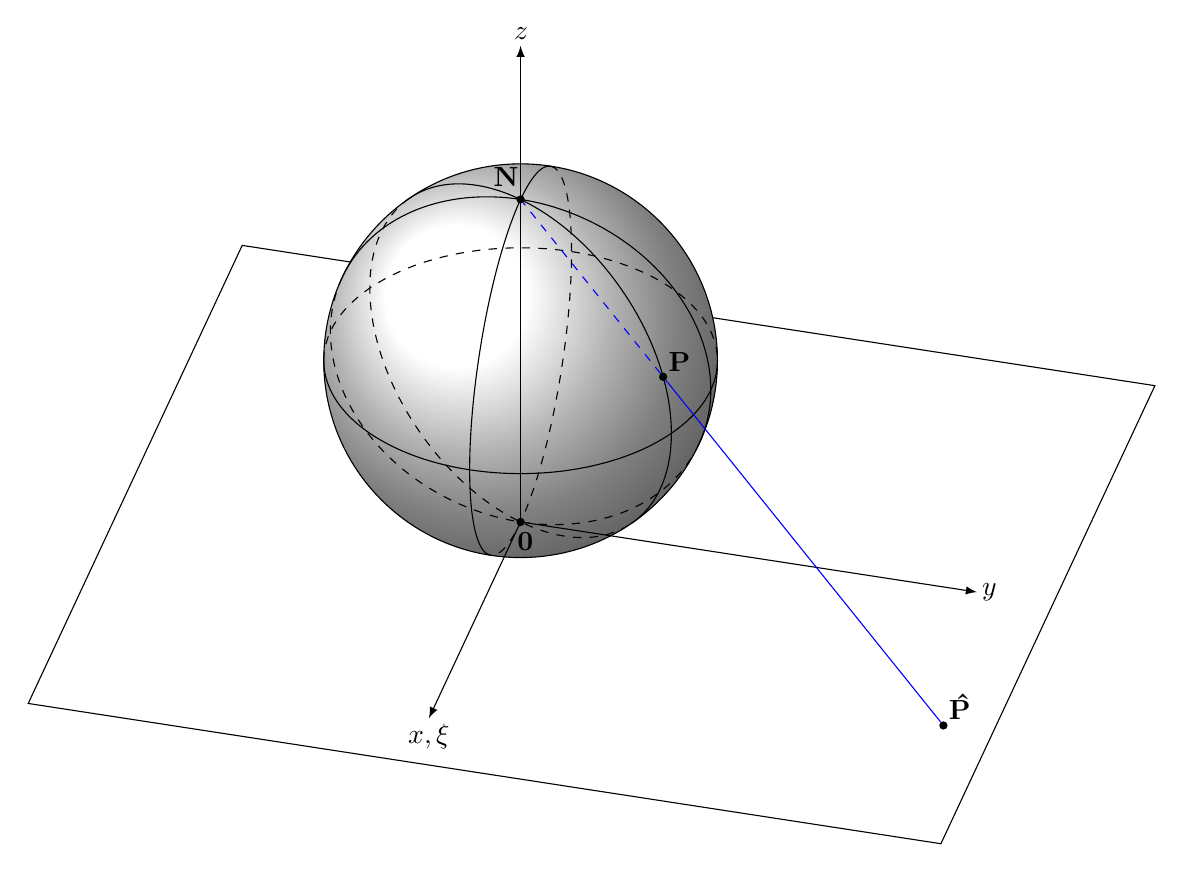
\begin{tikzpicture} % CENT
\newcommand\pgfmathsinandcos[3]{%
  \pgfmathsetmacro#1{sin(#3)}%
  \pgfmathsetmacro#2{cos(#3)}%
}
\newcommand\LongitudePlane[3][current plane]{%
  \pgfmathsinandcos\sinEl\cosEl{#2} % elevation
  \pgfmathsinandcos\sint\cost{#3} % azimuth
  \tikzset{#1/.estyle={cm={\cost,\sint*\sinEl,0,\cosEl,(0,0)}}}
}
\newcommand\LatitudePlane[3][current plane]{%
  \pgfmathsinandcos\sinEl\cosEl{#2} % elevation
  \pgfmathsinandcos\sint\cost{#3} % latitude
  \pgfmathsetmacro\yshift{\cosEl*\sint}
  \tikzset{#1/.estyle={cm={\cost,0,0,\cost*\sinEl,(0,\yshift)}}} %
}
\newcommand\DrawLongitudeCircle[2][1]{
  \LongitudePlane{\angEl}{#2}
  \tikzset{current plane/.prefix style={scale=#1}}
   % angle of "visibility"
  \pgfmathsetmacro\angVis{atan(sin(#2)*cos(\angEl)/sin(\angEl))} %
  \draw[current plane] (\angVis:1) arc (\angVis:\angVis+180:1);
  \draw[current plane,dashed] (\angVis-180:1) arc (\angVis-180:\angVis:1);
}
\newcommand\DrawLatitudeCircle[2][1]{
  \LatitudePlane{\angEl}{#2}
  \tikzset{current plane/.prefix style={scale=#1}}
  \pgfmathsetmacro\sinVis{sin(#2)/cos(#2)*sin(\angEl)/cos(\angEl)}
  % angle of "visibility"
  \pgfmathsetmacro\angVis{asin(min(1,max(\sinVis,-1)))}
  \draw[current plane] (\angVis:1) arc (\angVis:-\angVis-180:1);
  \draw[current plane,dashed] (180-\angVis:1) arc (180-\angVis:\angVis:1);
}

\tikzset{%
  >=latex, % option for nice arrows
  inner sep=0pt,%
  outer sep=2pt,%
  mark coordinate/.style={inner sep=0pt,outer sep=0pt,minimum size=3pt,
    fill=black,circle}%
}
%% some definitions

\def\R{2.5} % sphere radius
\def\angEl{35} % elevation angle
\def\angAz{-105} % azimuth angle
\def\angPhi{-40} % longitude of point P
\def\angBeta{19} % latitude of point P

%% working planes

\pgfmathsetmacro\H{\R*cos(\angEl)} % distance to north pole
\tikzset{xyplane/.estyle={cm={cos(\angAz),sin(\angAz)*sin(\angEl),-sin(\angAz),
                              cos(\angAz)*sin(\angEl),(0,-\H)}}}
\LongitudePlane[xzplane]{\angEl}{\angAz}
\LongitudePlane[pzplane]{\angEl}{\angPhi}
\LatitudePlane[equator]{\angEl}{0}

%% draw xyplane and sphere

\draw[xyplane] (-2*\R,-2*\R) rectangle (2.2*\R,2.8*\R);
\fill[ball color=white] (0,0) circle (\R); % 3D lighting effect
\draw (0,0) circle (\R);

%% characteristic points

\coordinate (O) at (0,0);
\coordinate[mark coordinate] (N) at (0,\H);
\coordinate[mark coordinate] (S) at (0,-\H);
\path[pzplane] (\angBeta:\R) coordinate[mark coordinate] (P);
\path[pzplane] (\R,0) coordinate (PE);
\path[xzplane] (\R,0) coordinate (XE);
\path (PE) ++(0,-\H) coordinate (Paux); % to aid Phat calculation
\coordinate[mark coordinate] (Phat) at (intersection cs: first line={(N)--(P)},
                                        second line={(S)--(Paux)});

%% draw meridians and latitude circles

\DrawLatitudeCircle[\R]{0} % equator
\DrawLongitudeCircle[\R]{\angAz} % xzplane
\DrawLongitudeCircle[\R]{\angAz+90} % yzplane
\DrawLongitudeCircle[\R]{\angPhi} % pzplane

%% draw xyz coordinate system

\draw[xyplane,<->] (1.8*\R,0) node[below] {$x,\xi$} -- (0,0) -- (0,2.4*\R)
    node[right] {$y$};
\draw[->] (0,-\H) -- (0,1.6*\R) node[above] {$z$};

%% draw lines and put labels

\draw[blue,dashed] (P) -- (N) +(0.3ex,0.6ex) node[above left,black] {$\mathbf{N}$};
\draw[blue] (P) -- (Phat) node[above right,black] {$\mathbf{\hat{P}}$};
\path (S) +(0.4ex,-0.4ex) node[below] {$\mathbf{0}$};
\draw (P) node[above right] {$\mathbf{P}$};
\end{tikzpicture}
   \end{center}
\end{examplle}

By a \textbf{disc} we mean any space homeomorphic to the closed unit disc \(D\) in
\(\R^2\). \(C\) stands for the unit circle. If \(A\) is a disc, and if
\(h:A\to D\) is a homeomorphism, then \(h^{-1}(C)\) is called the \textbf{boundary} of
\(A\) and is written \(\partial A\).

\begin{lemma}[]
\label{lemma2.10}
Any homeomorphism from the boundary of a disc to itself can be extended to a
homeomorphism of the whole disc
\end{lemma}

\begin{proof}
Let \(A\) be a disc and choose a homeomorphism \(h:A\to D\). Given a
homeomorphism \(g:\partial A\to\partial A\), we can easily extend \(hgh^{-1}:C\to
   C\) to a homeomorphism of all of \(D\)as follows. Send 0 to 0, and if \(x\in
   D-\{0\}\) send \(x\) to the point \(\norm{x}hgh^{-1}(x/\norm{x})\). In other
words extend conically
\end{proof}

\begin{lemma}[]
Let \(A\) and \(B\) be discs which intersect along their boundaries in an
arc. Then \(A\cup B\) is a disc.
\end{lemma}

\begin{proof}
Let \(\gamma\) denote the arc \(A\cap B\), and use \(\alpha\), \(\beta\) for the complementary arcs in
the boundaries of \(A\) and \(B\). We construct a homeomorphism from \(A\cup
   B\) to \(D\) with the aid of lemma \ref{lemma2.10}

The \(y\) axis in the plain divides up \(D\) as the union of two discs
\(D_1\) and \(D_2\). We label the three arcs which together make up the
boundaries of \(D_1\) and \(D_2\) as \(\alpha'\), \(\beta'\) and \(\gamma'\).
Both \(\alpha\) and \(\alpha'\) are homeomorphic to the clsoed unit interval
\([0,1]\), so we can find a homeomorphism from \(\alpha\) to \(\alpha'\). We first
extend this over \(\gamma\), to give a homeomorphism from \(\alpha\cup\gamma\) to
\(\alpha'\cup\gamma'\); then over \(A\) to give a homeomorphism from \(A\) to
\(D_1\), which take \(\gamma\) to \(\gamma'\), using lemma \ref{lemma2.10}.
\end{proof}


\subsubsection{Exercise}
\label{sec:org0c32276}
\begin{exercise}
\label{ex2.13}
If \(f:\R\to\R\) is a map, show that the set of points which are left fixed
by \(f\) is a closed subset of \(\R\). If \(g\) is a continuous real-valued
function on \(X\) show that the set \(\{x\mid g(x)=0\}\) is closed
\end{exercise}

\begin{proof}
Define \(f_0(x)=f(x)-x\)
\end{proof}

\begin{exercise}
\label{ex2.25}
Let \(f:\R\to\R\) be a map and define its graph \(\Gamma_f:\R\to\R^2\) by
\(\Gamma_f(x)=(x,f(x))\). Show that \(\Gamma_f\) is continuous and that its
image (taken with the topology induced from \(\R^2\)) is homeomorphic to \(\R\)
\end{exercise}

\begin{proof}
The function \(p_1:\im\Gamma_f\to\E\) defined by \((x,f(x)\mapsto x)\) is
the desired homeomorphism
\end{proof}

\begin{exercise}
\label{ex2.16}
What topology must \(X\) have if every real-valued function defined on \(X\)
is continuous
\end{exercise}

\begin{proof}
Discrete topology. It suffices to show points in \(X\) are open

Fix \(x\in X\) and define \(f:X\to\R\) by
\begin{equation*}
f(x)=
\begin{cases}
f(x)=0\\
f(y)=1&y\neq x
\end{cases}
 \end{equation*}
Then \(f^{-1}((-0.5,0.5))=\{x\}\)
\end{proof}

\begin{exercise}
An \textbf{open map} is one which sends open sets to open sets: a \textbf{closed map} takes
closed sets to closed sets. Which of the following maps are open or closed
\begin{enumerate}
\item The exponential map \(x\mapsto e^{ix}\) from the real line to the circle
\item The folding map \(f:\R^2\to\R^2\) given by \((x,y)\mapsto(x,\abs{y})\)
\item The map which winds the plane three times on itself given in terms of
complex numbers, by \(z\mapsto z^3\)
\end{enumerate}
\end{exercise}

\begin{proof}
\begin{enumerate}
\item 

\item not open. closed.
\item open. closed
\end{enumerate}
\end{proof}
\subsection{A space-filling curve}
\label{sec:orgdeb4cf4}
\subsection{The Tietze extension theorem}
\label{sec:org67e3bc0}
Let \(X\) be a topological space and \(A\) a subspace of \(X\). Given a
real-valued continuous function defined on \(A\), it is natural to ask
whether or not we can always extend it to all of \(X\).

\begin{definition}[]
A \textbf{metric} or \textbf{distance function} on a set \(X\) is a real-valued function \(d\)
defined on the cartesian product \(X\times X\) s.t. for all \(x,y,z\in X\)
\begin{enumerate}
\item \(d(x,y)\ge0\) with equality iff \(x=y\)
\item \(d(x,y)=d(y,x)\)
\item \(d(x,y)+d(y,z)\ge d(x,z)\)
\end{enumerate}


A set together with a metric on it is called a \textbf{metric space}
\end{definition}

A metric on a set gives rise to a topology on the set as follows. Let \(d\)
be a metric on the set \(X\). Given \(x\in X\), the set \(\{y\in X\mid
   d(x,y)\}\le\epsilon\) is called the \textbf{ball of radius} \(\epsilon\), or
\(\epsilon\)-ball, centered at the point \(x\), and is denoted by \(B(x,\epsilon)\).
We define a subset \(O\) of \(X\) to be \textbf{open} if given \(x\in O\) we can find
a positive real number \(\epsilon\) s.t. \(B(x,\epsilon)\subset O\).

Different metrics on a set may give the same topology. For example, we can
make the underlying set of points of euclidean \(n\)-space into a metric
space in three different ways as follows. Write
\(\bx=(x_1,\dots,x_n)\in\R^n\), define:
\begin{enumerate}
\item \(d_1(\bx,\by)=\sqrt{(x_1-y_1)^2+\dots+(x_n-y_n)^2}\)
\item \(d_2(\bx,\by)=\max_{1\le i\le n}\abs{x_i-y_i}\)
\item \(d_3(\bx,\by)=\abs{x_1-y_1}+\dots+\abs{x_n-y_n}\)
\end{enumerate}


Following shows the ball of radius 1, centered at the origin for each of
these three metrics when \(n=2\).

\begin{center}
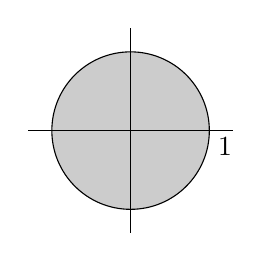
\begin{tikzpicture}
\draw[fill=black!20,draw=Black] (0,0) circle [radius=1cm];
   \draw (-1.3,0) -- (1.3,0);
\draw (0,-1.3) -- (0,1.3);
\node at (1.2,-0.2) {1};
\end{tikzpicture}
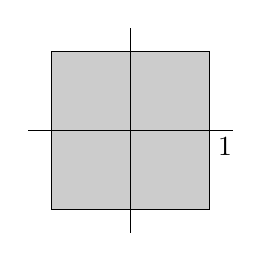
\begin{tikzpicture}
\draw[fill=black!20] (-1,-1) rectangle (1,1);
\draw (-1.3,0) -- (1.3,0);
\draw (0,-1.3) -- (0,1.3);
\node at (1.2,-0.2) {1};
\end{tikzpicture}
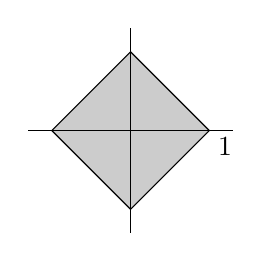
\begin{tikzpicture}
\draw[fill=black!20] (-1,0) -- (0,1) -- (1,0) -- (0,-1) -- (-1,0);
\draw (-1.3,0) -- (1.3,0);
\draw (0,-1.3) -- (0,1.3);
\node at (1.2,-0.2) {1};
\end{tikzpicture}
\end{center}

To see that \(d_1\) and \(d_2\) give rise to the same topology, we note that
inside any disc we can find a square, and conversely inside a square we can
find a disc.

Given two distinct points in a metric space, we can always find disjoint open
sets containing them. For if \(d(x,y)=\delta>0\), set \(U=\{z\in X\mid
   d(x,z)<\delta/2\}\) and \(V=\{z\in X\mid d(y,z)\le\delta/2\}\). Then both
\(U\) and \(V\) are open sets. The set \(U\) is usually called the \textbf{open ball}
with center \(x\) and radius \(\delta/2\). A topological space with the
property that two distinct points can always be surrounded by disjoint open
sets is called a \textbf{Hausdorff space}.

If \(d\) is a metric on \(X\) and if \(A\) is a subset of \(X\), the distance
\(d(x,A)\) of the point \(x\) from \(A\) is defined to be the infimum of the
numbers \(d(x,a)\) where \(a\in A\)

\begin{lemma}[]
The real-valued function on \(X\) defined by \(x\mapsto d(x,A)\) is continuous
\end{lemma}

\begin{proof}
Let \(x\in X\) and let \(N\) be a neighbourhood of \(d(x,A)\) on the real
line. Choose \(\epsilon>0\) small enough so that the interval
\((d(x,A)-\epsilon,d(x,A)+\epsilon)\) lies inside \(N\). Let \(U\) denote the
open ball centered \(x\), radius \(\epsilon/2\), \(z\in U\), and choose a point \(a\in
   A\) s.t.
\(d(x,a)<d(x,A)+\epsilon/2\). If \(z\in U\) we have
\begin{equation*}
d(z,A)\le d(z,a)\le d(z,x)+d(x,a)<d(x,A)+\epsilon
\end{equation*}
By reversing the roles of \(x\) and \(z\), we also have
\(d(x,A)<d(z,A)+\epsilon\). Therefore \(U\) is mapped inside
\((d(x,A)-\epsilon,d(x,A)+\epsilon)\) and hence inside \(N\), by our
function, showing that the inverse image of \(N\) is a neighbourhood of \(x\)
in \(X\) as required.
\end{proof}

\begin{lemma}[]
If \(A,B\) are disjoint closed subsets of a metric space \(X\), there is a
continuous real-valued function on \(X\) which takes the value 1 on points of
\(A\), -1 on points of \(B\), and values strictly between \(\pm1\) on points
of \(X-(A\cup B)\)
\end{lemma}

\begin{proof}
Since \(A\) and \(B\)
\end{proof}
















\subsubsection{Exercise}
\label{sec:orgfbe928e}
\begin{exercise}
\label{ex2.4.27}
Show \(d(x,A)=0\) iff \(x\) is a point of \(\bbar{A}\)
\end{exercise}

\begin{proof}
Suppose that \(d(x,A)=0=\inf_{a\in A}d(x,a)\). Then for every \(\epsilon>0\), there
exists \(a\in A\) s.t.
\begin{equation*}
\abs{d(x,a)-0}=d(x,a)<\epsilon
\end{equation*}
Now let \(\calo\) be an open subset of \(X\), \(x\in\calo\). Choose \(a\in
    A\) s.t. \(d(x,a)<\epsilon\). Then \(a\in\calo\) and \(\calo\cap
    A\neq\emptyset\). Thus \(x\in\bbar{A}\)

Suppose that \(x\in\bbar{A}\). Then we do the canonical ball construction
and pick a sequence \(\{a_n\}_n\) of elements of \(A\), s.t.
\(d(x,a_n)\to0\), \(n\to\infty\)
\end{proof}
\end{document}
